\documentclass[a4paper, 11pt]{article}
\usepackage[utf8]{inputenc}
\usepackage{float}
\usepackage{graphicx}
\usepackage{url}
\usepackage{enumitem}
\usepackage{subcaption}

\setlist[itemize]{itemsep=0.5pt, parsep=0.5pt, topsep=0pt, partopsep=0pt}
\setlist[enumerate]{itemsep=0.5pt, parsep=0.5pt, topsep=0pt, partopsep=0pt}

%opening
\title{HW2 Report, Rudy: A Small Routing Protocol}
\author{David Fischer}
\date{\today{}}

\begin{document}

\maketitle

\section{Introduction}

\textit{Summary of the work you've done, what are the topics we cover
  in this seminar, etc. Remember that you should deliver this report
  at the start of the seminar.}

What is the main topic related to distributed systems covered in this seminar?
Why is it important?

\section{Main problems and solutions}

\subsection{Module Based Approach}

\subsection{Debugging Final Implementation}

\textit{Summarize your problems, proposed solutions, etc. You do not
  need to copy\&paste your code. Only if needed, you may write down
  small code snipeds to show how you have solved a specific
  problem/question.}

Did you find any specific problem with the development of your
solution?  How did you solve it?

\begin{verbatim}
this(X) ->
    Y = is(X),
    a(test(Y)).
\end{verbatim}

\section{Evaluation}

\textit{If needed, you may provide figures or tables with main results
  evaluating your proposals. For each seminar, we will provide you
  with some guidance on which kind of evaluation you should do.}

Figure \ref{fig:map1}
\begin{figure}[H]
  \begin{center}
    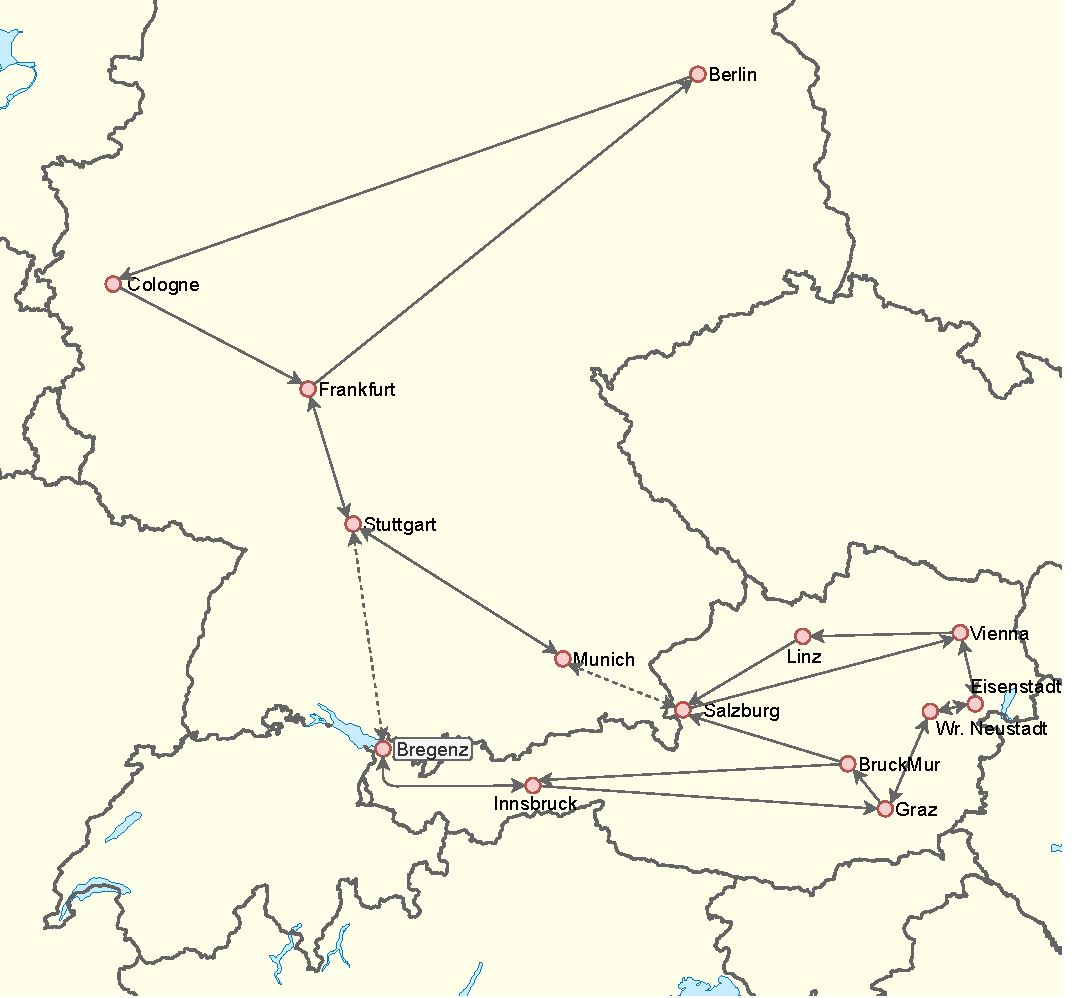
\includegraphics[width=\textwidth]{graphics/map_routy.pdf}
    \caption{Map of routers used for evaluation}
    \label{fig:map1}
  \end{center}
\end{figure}

\section{Conclusions}

What have you learnt from the problem presented?
Was it useful?

\end{document}
